\documentclass{beamer}
\mode<presentation>{\usetheme{boxes}}
\usepackage[T1]{fontenc}
\usepackage{amsmath}
\usepackage{times}
\usepackage{color}
\usepackage{graphicx}
\usepackage[utf8x]{inputenc}

\title{Rameau: Automatic Harmonic Analysis}
\author{Pedro Kröger and Alexandre Passos}

\beamersetaveragebackground{black}
\setbeamercolor{normal text}{fg=white} 

\begin{document}

\maketitle

\begin{frame}
  \frametitle{The process is:}
  \framesubtitle{from a score parse it into a list of events and
    simplify to a list of pitches}
  \addvspace{2.5em}
   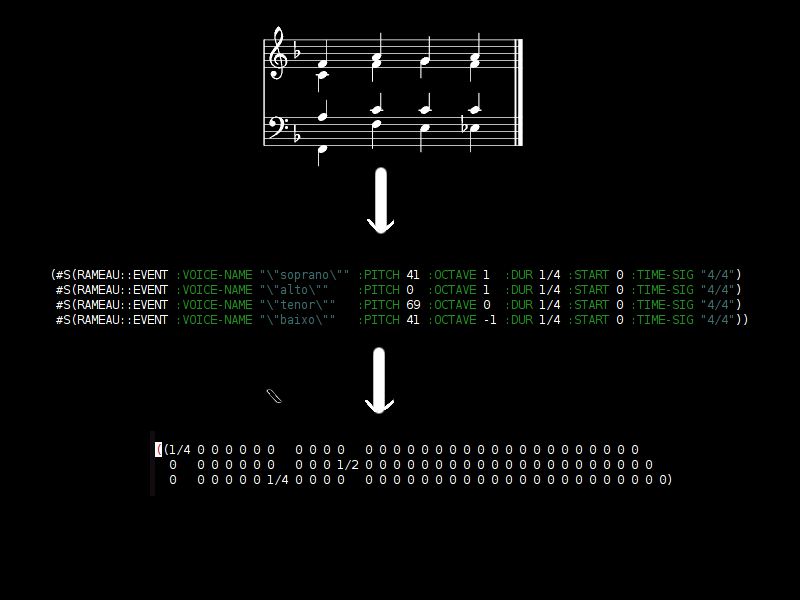
\includegraphics[scale=0.45, trim = 5em 0cm 0cm 4em]{figs/process}
\end{frame}


\begin{frame}
  \frametitle{Each algorithm}
  \framesubtitle{converts the list of pitches into chords}
  \centering
  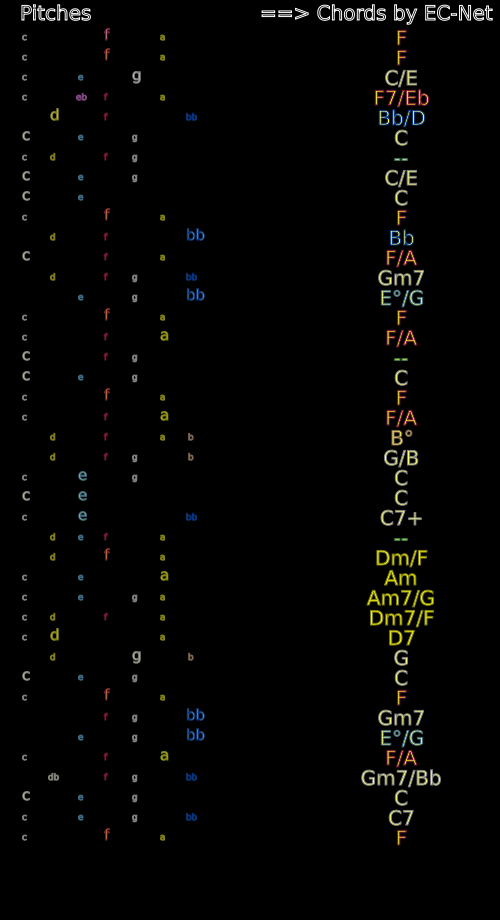
\includegraphics[scale=0.6, trim = 0em 51em 0em 0em, clip ]{figs/algorithm}
\end{frame}

\begin{frame}
  \frametitle{But... how?}
  \framesubtitle{Pardo and Birmingham's algorithm: straight
    template-matching}
  \begin{center}
    \begin{tabular}{rrr}
      0 &            &  \\
      4 & $\implies$ & Major \\
      7 &            &  \\ 
      \hline
      0 &            &  \\
      3 & $\implies$ & Minor \\
      7 &            &  \\
    \end{tabular}
  
    And so on\footnote{But we did extend it to have enough labels and
      be enharmonically savvy}\ldots
  \end{center}
\end{frame}

\begin{frame}
  \frametitle{But... how?}
  \framesubtitle{Temperley and Sleator's algorithm:
    maximizing something over the piece}
  \begin{center}
    \begin{huge}
      Too slow.
    \end{huge}
    
    \addvspace{5em}
    And too complex. And also too wrong, so we took it out.

  \end{center}
\end{frame}


\begin{frame}
  \frametitle{But... how?}
  \framesubtitle{Naïve bayesian algorithm: the chord that gives the highest
    probability to each sonority}
  \addvspace{0.5em}
  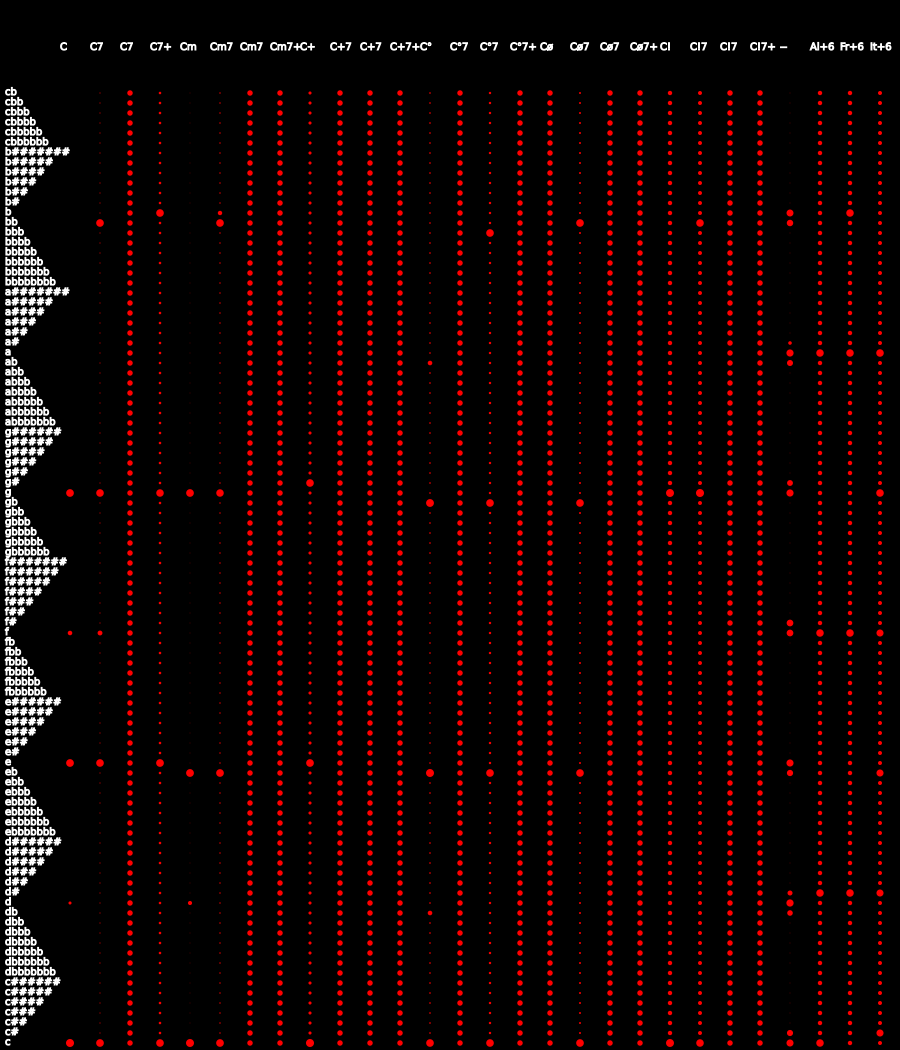
\includegraphics[scale=0.4, trim = 6em 0 0 0]{figs/notesprobs}
\end{frame}

\begin{frame}
  \frametitle{But... how?}
  \framesubtitle{Hidden Markov Model: Like the bayesian, but
    maximizing the probability of the entire piece in a Markov Model}
  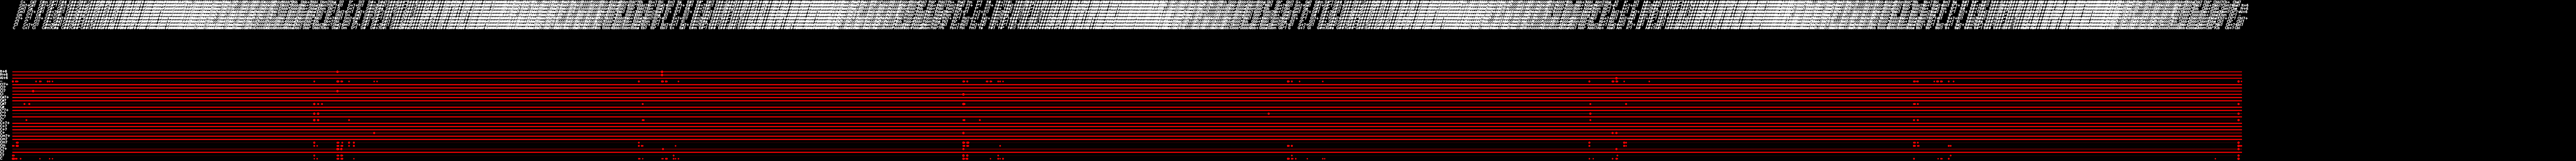
\includegraphics[scale=0.4, trim = 6em 0 0 0]{figs/transprobs}
\end{frame}

\begin{frame}
  \frametitle{But... how?}
  \framesubtitle{K-Nearest Neighbors algorithm: the most common chord
    label closest to the pitches being analyzed (these are the ones for a C E G chord)}
  \addvspace{0.5em}
  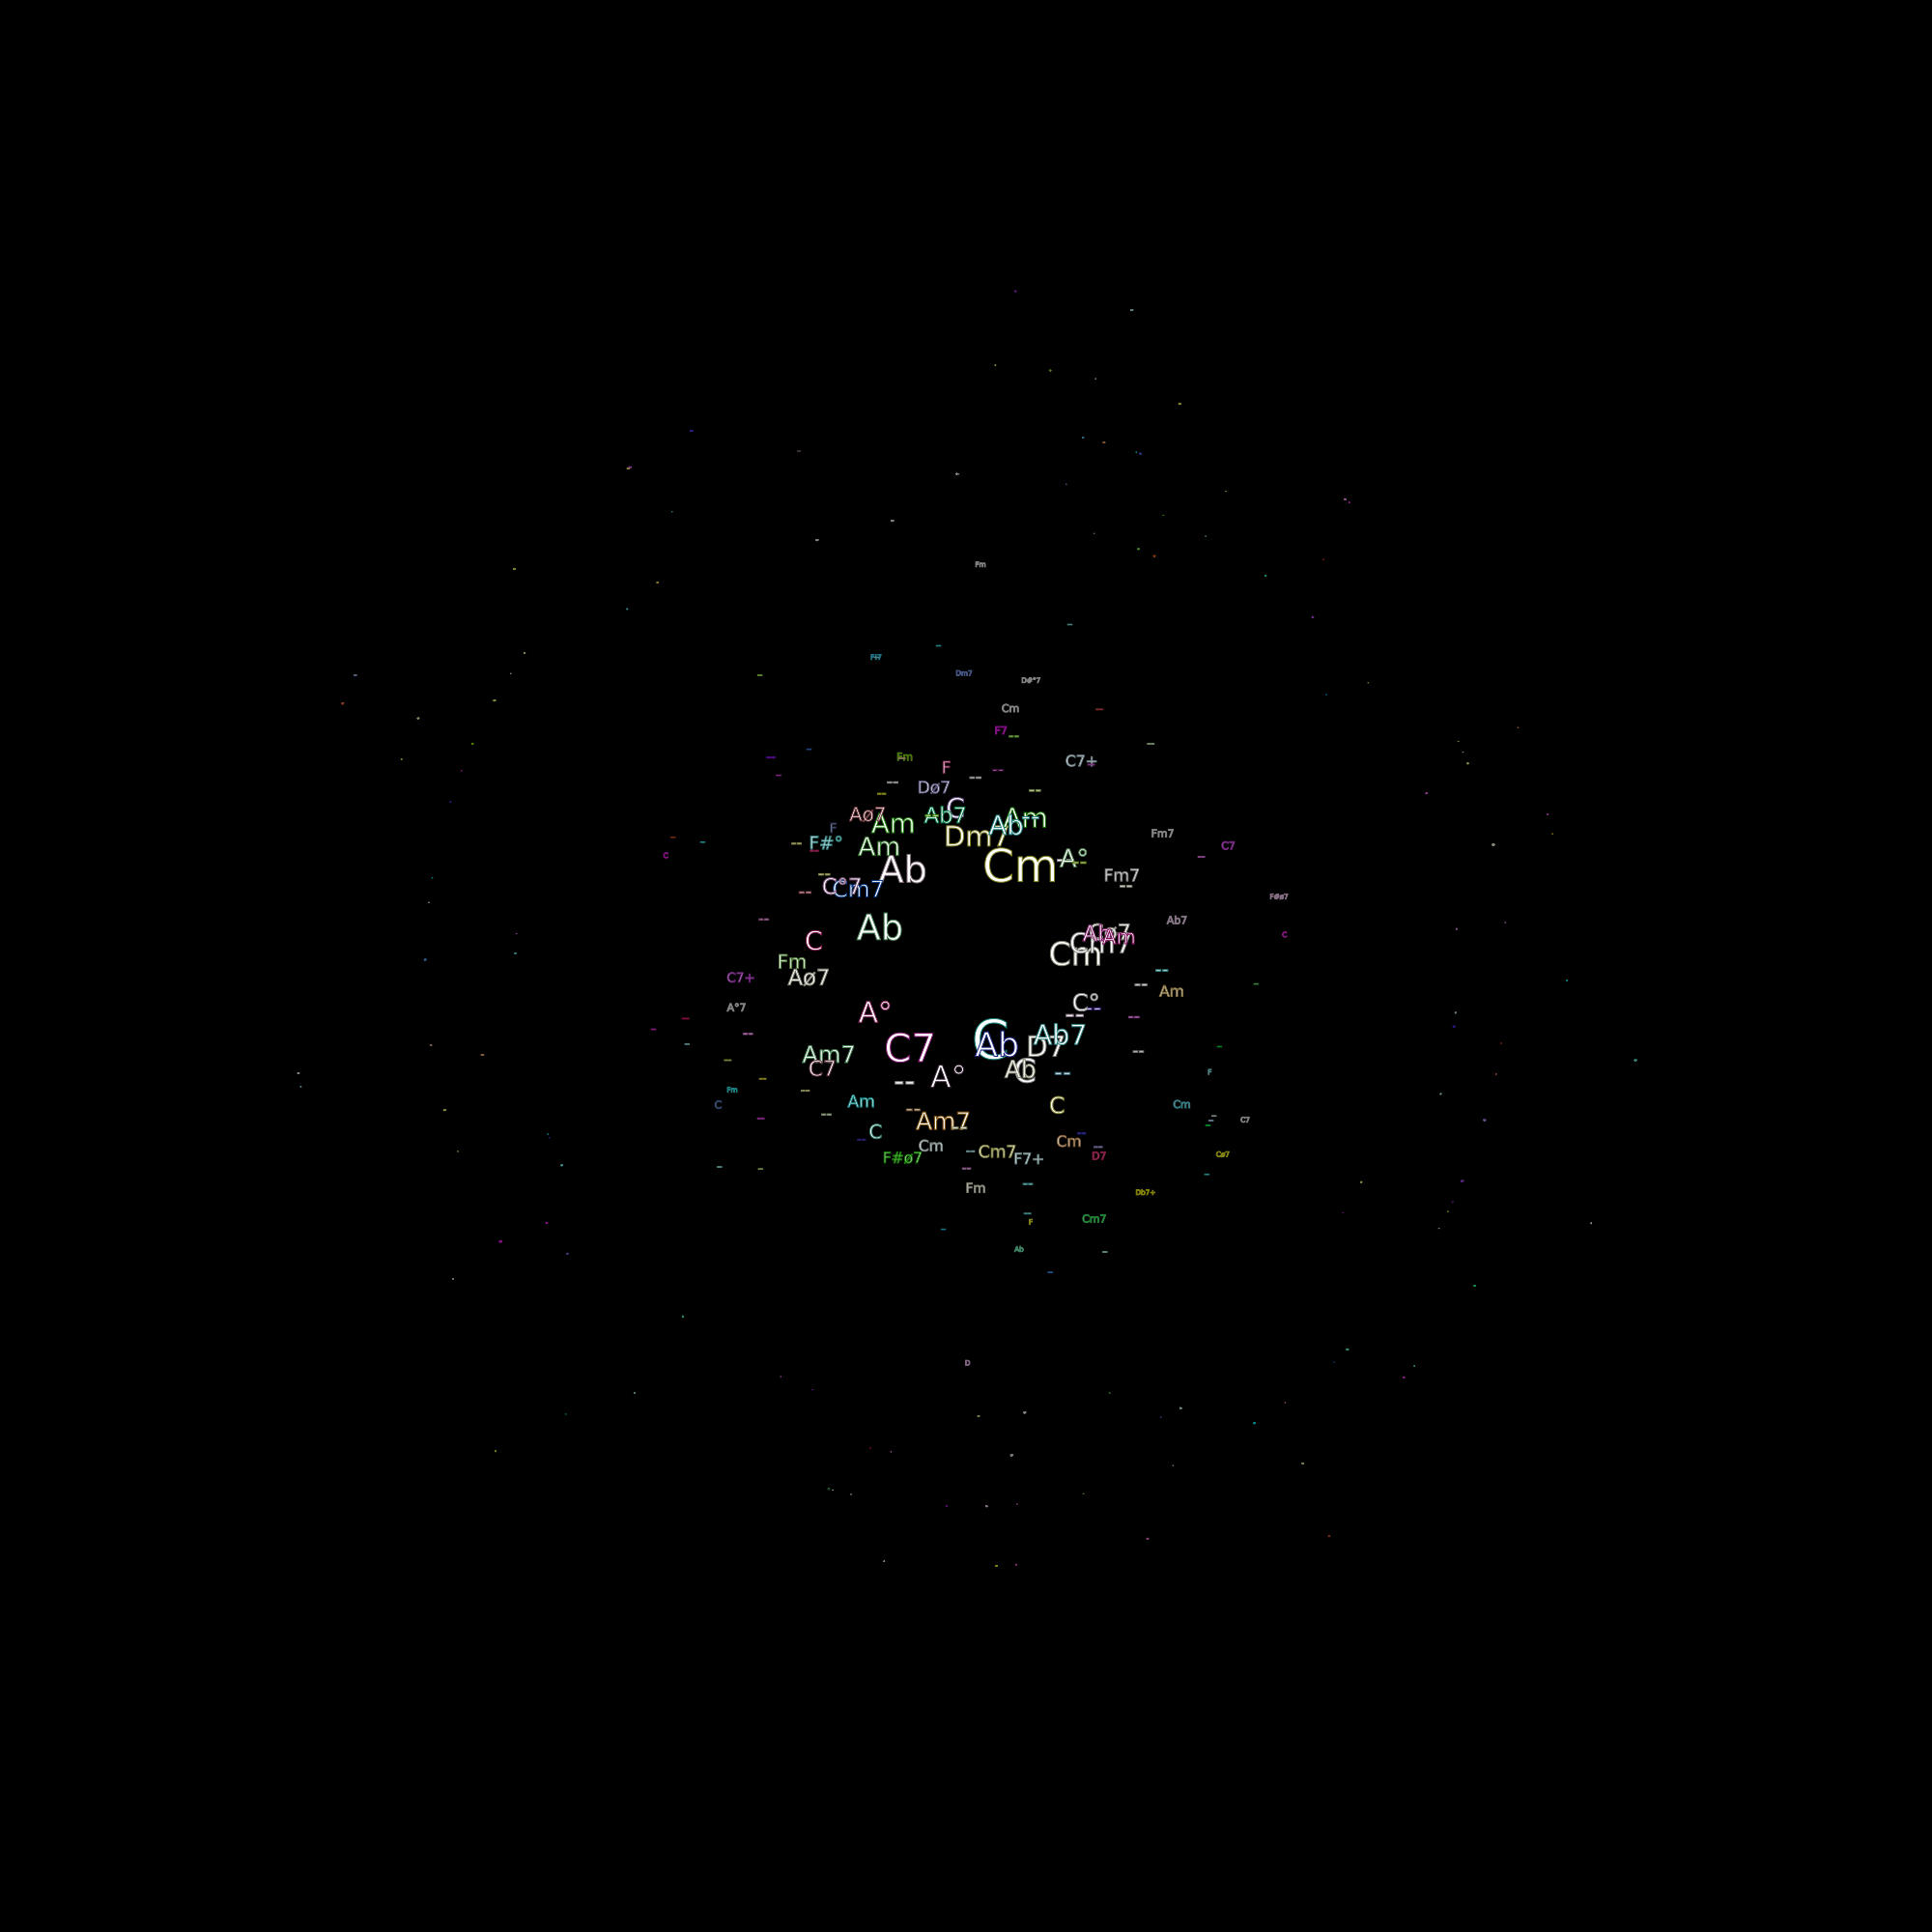
\includegraphics[scale=0.3, trim = 50em 0em 0em 51em, clip]{figs/knn}
\end{frame}

\begin{frame}
  \frametitle{But... how?}
  \framesubtitle{Decision tree: implicit rule-following}
    \begin{large}
      If first pitch is 0 and second pitch is 28 and third pitch is
      55\footnote{That's for a C E G chord, by the way}, then the chord is a C
      major.

      \addvspace{1em}

      If first pitch is 0 and second pitch is 27 and third pitch is
      55\footnote{And that's for a C E$\flat$ G chord}, then the chord is a C
      minor.
    \end{large}
  \begin{center}

    \addvspace{3em}

    And so on...%
  \end{center}
\end{frame}


\begin{frame}
  \frametitle{But... how?}
  \framesubtitle{Neural networks (Tsui): pattern-matching over each sonority's
  pitches}

Neural networks work by doing...
\pause

I mean, it's easy, they just...
\pause

Well, they're very good, right?

\pause
\addvspace{2em}
\begin{small}
  Currently the best algorithm is a neural network that only looks at
  one sonority at a time. \pause Go figure.
\end{small}
\end{frame}


\begin{frame}
  \frametitle{Cadence detection:}
  \framesubtitle{these are all the final cadences in the Bach chorales}
  \centering
  \addvspace{0.5em}
  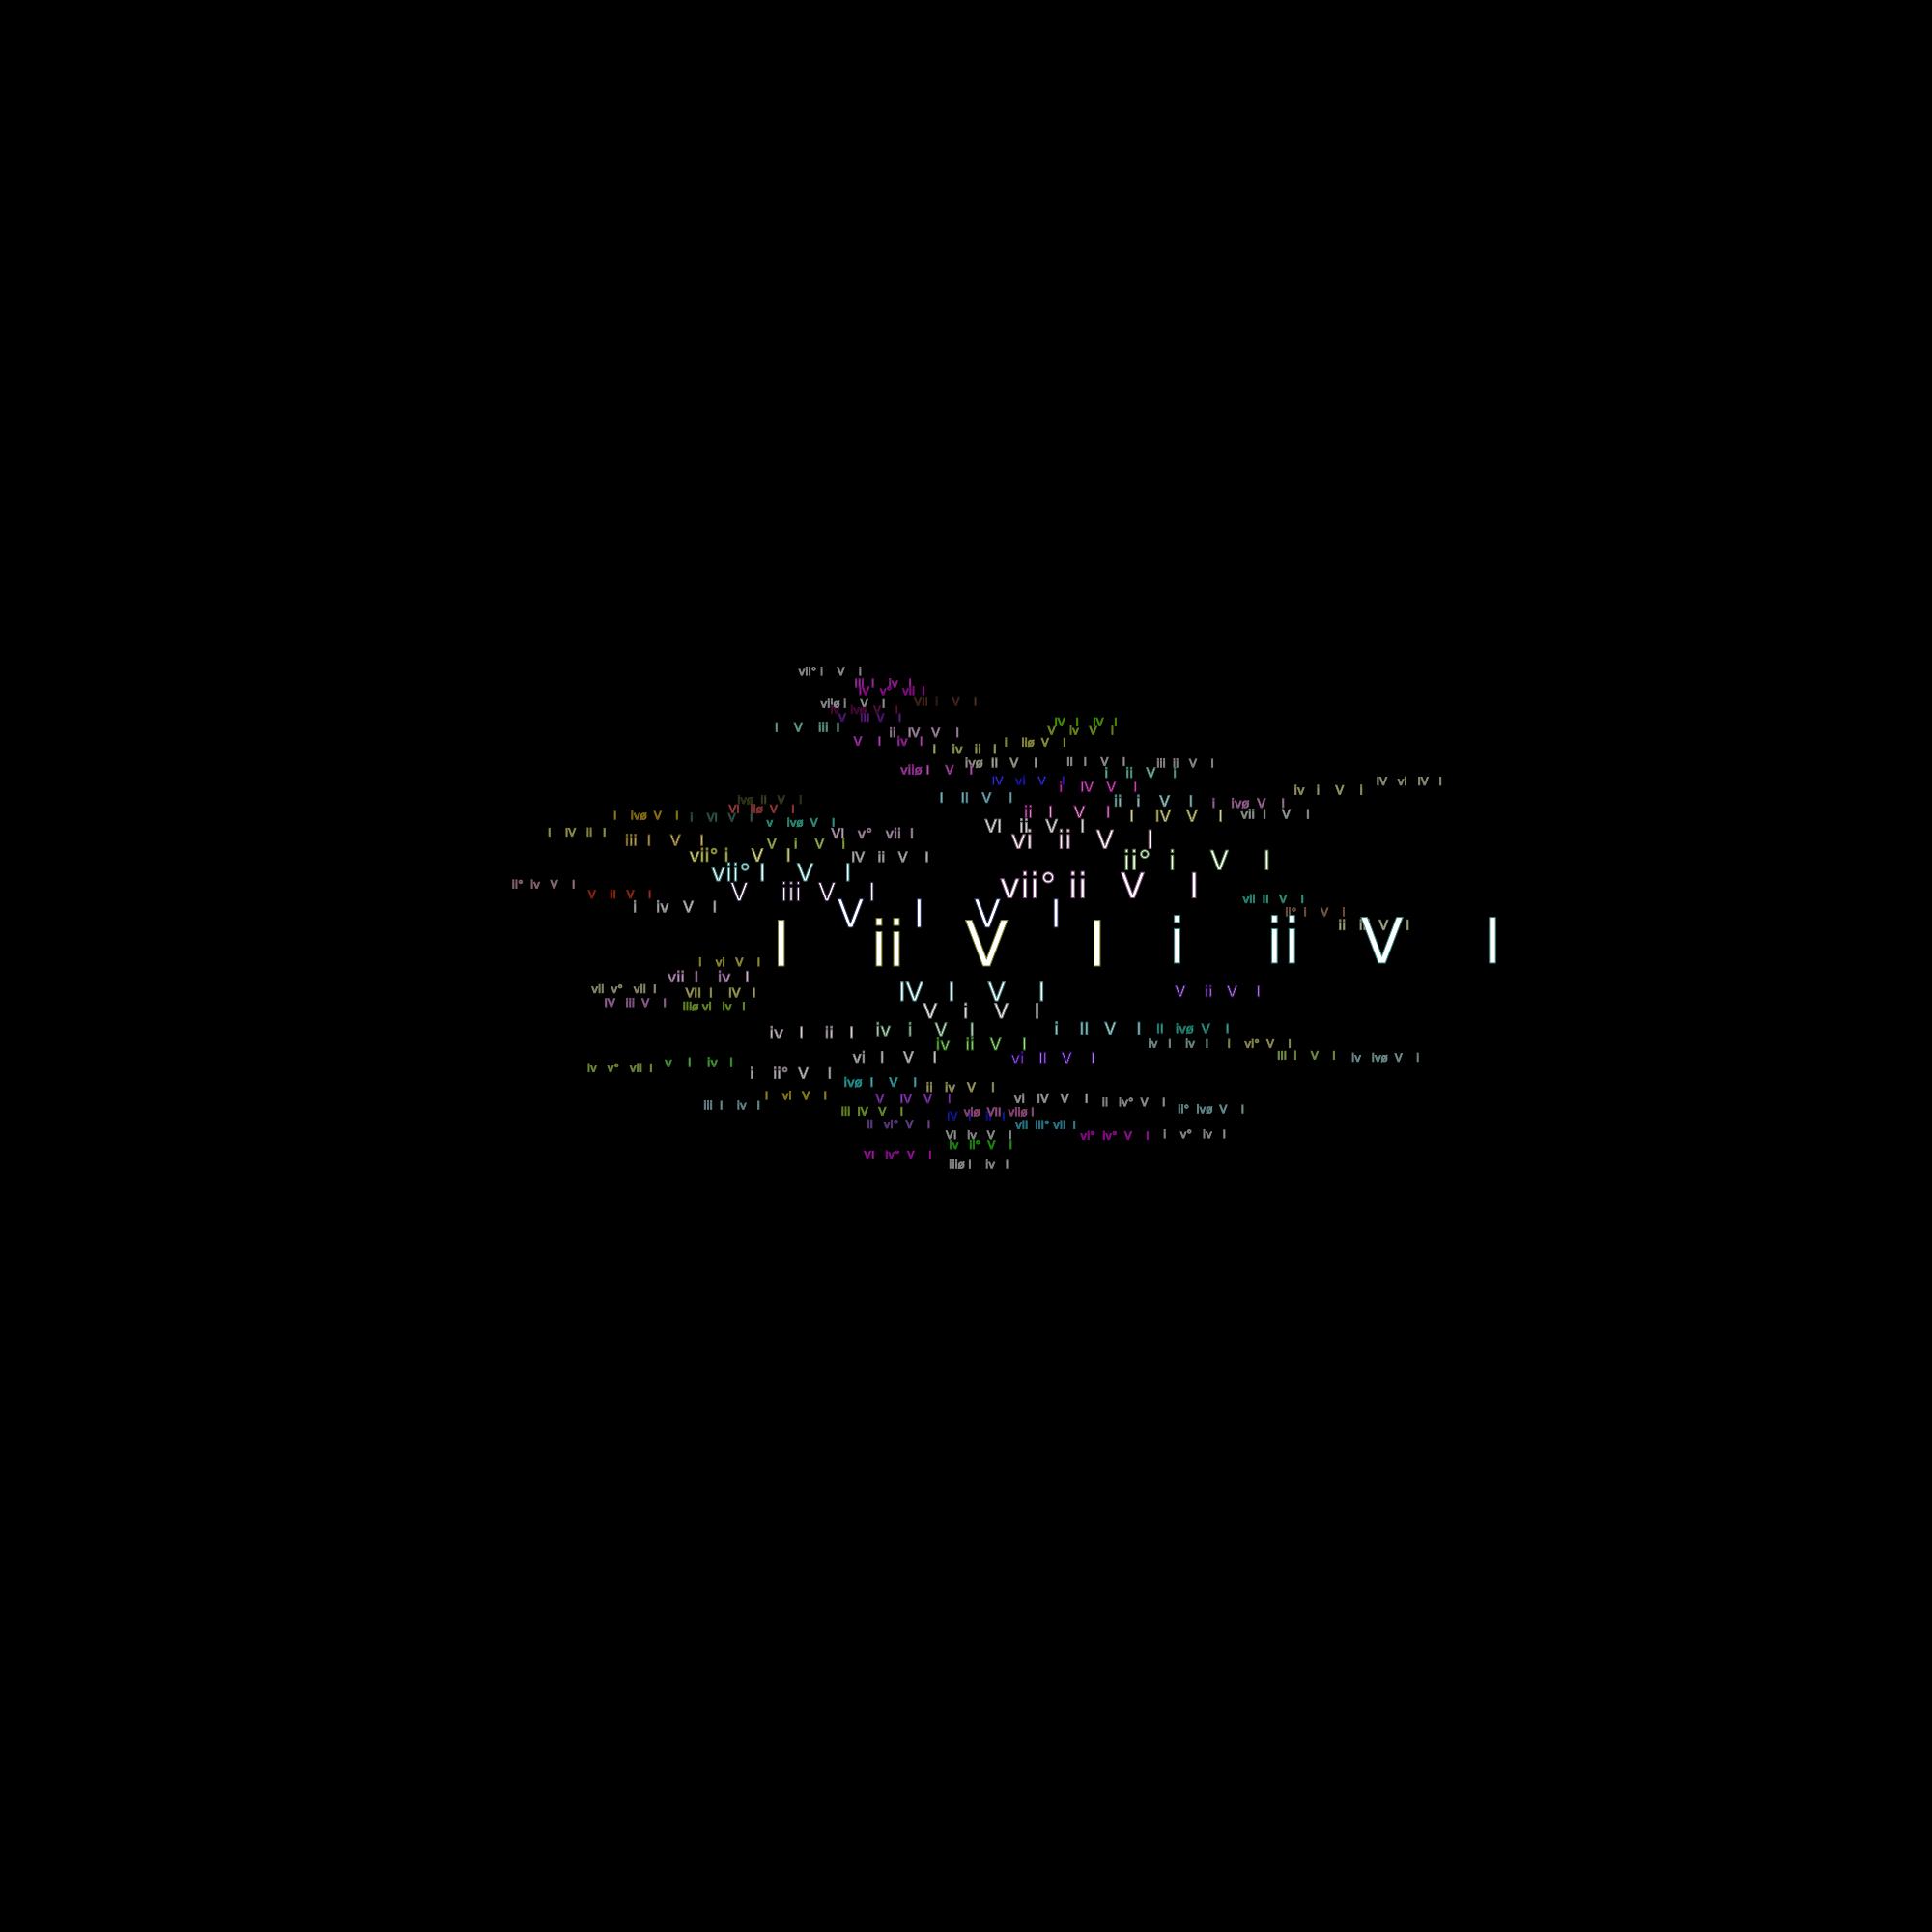
\includegraphics[scale=0.3, trim = 50em 0em 0em 50em, clip]{figs/cadences}
\end{frame}



\begin{frame}
  \frametitle{The end.}
  \framesubtitle{Questions?\footnote{No artists were harmed in the making of this presentation:
    all the cool figures were automatically generated, using the
    Vecto library and GNU Lilypond}}
  \centering
  
\includegraphics[scale=0.3, trim = -25em 0em 0em 0em]{figs/genos}
\end{frame}


\end{document}
